%-------------------------------------------------------------------------------
% File: Report.tex
% Author: Igor Janjic, Danny Duangphachanh, Leah Krynitsky, Brian
% Hilnbrand
% Description: [ECE 4534] Embedded Systems Design
% Project proposal.
%%------------------------------------------------------------------------------ 


%-------------------------------------------------------------------------------
% File:		Preamble.tex
% Author:	Igor Janjic
% Description:	Defines which packages to use.
%%------------------------------------------------------------------------------

\documentclass[11pt]{article}

% Encodes font as T1.
\usepackage[T1]{fontenc}

% Pretty much all of the ams maths packages.
\usepackage{amsmath,amsthm,amssymb,amsfonts}

% Allows you to manipulate the page a bit.
\usepackage[margin=0.75in]{geometry}

% Removes paragraph indentation.
\usepackage{parskip}

% Allows inclusion of graphics easily.
\usepackage{graphicx}

% Provides ways to make nice looking tables.
\usepackage{booktabs}

% Allows rotation of tables and figures.
\usepackage{rotating}

% Allows color.
\usepackage{color}

% Allows shading of table cells.
\usepackage{colortbl}

% Allows hyphenatable letterspacing, underlining, and highlighting.
\usepackage{soul}

% Allows extra text symbols.
\usepackage{textcomp}

% Allows manipulation of floats.
\usepackage{float}

% Provides commands to make subfigures.
\usepackage{subfigure}

% Typesets URLs sensibly with tt font, clickability in PDFs, and not breaking across lines.
\usepackage{url}

% Makes references hyperlinks in PDF output.
\usepackage{hyperref}

% Provides good access to colors.
\usepackage{color}

% Provides good access to colors.
\usepackage{xcolor}

% Provides for programming code to be inserted into the document.
\usepackage{listings}

% Provides support for table coloring.
\usepackage{xcolor}

% Provides vector graphics functionality.
\usepackage{tikz}
\usetikzlibrary{shapes.geometric, arrows, positioning}

% Provides circuit vector graphics functionality.
\usepackage{circuitikz}

% Provides caption manipulation.
\usepackage{caption}

% Makes sure tables don't float about if they have the designation [H].
\restylefloat{table}

% Defines the color gray.
\definecolor{gray}{rgb}{0.5, 0.5, 0.5}


%-------------------------------------------------------------------------------
% File:		Definitions.tex
% Author:	Igor Janjic
% Description:	Contains various commands.
%%------------------------------------------------------------------------------

%-------------------------------------------------------------------------------
% General Definitions

% Defines a command for skipping a line.
\def\wl{\par\vspace{\baselineskip}}

% Defines a command for hiding text.
\newcommand{\hide}[1]{}

% Defines a command for a shortened commonly used phrases.
\newcommand{\ie}{\text{i.e.}}
\newcommand{\eg}{\text{e.g.}}
\newcommand{\ex}{\text{e.x.}}
\newcommand{\ans}{\textbf{Answer: }}
\newcommand{\pro}{\textbf{Proof: }}

% Defines a command to mark to-do items in red.
\newcommand{\todo}[1] {\textbf{\textcolor{red}{#1}}}

% Defines commands for calligraphic font.
\newcommand{\calA}{\mathcal{A}}
\newcommand{\calB}{\mathcal{B}}
\newcommand{\calC}{\mathcal{C}}
\newcommand{\calD}{\mathcal{D}}
\newcommand{\calE}{\mathcal{E}}
\newcommand{\calF}{\mathcal{F}}
\newcommand{\calG}{\mathcal{G}}
\newcommand{\calH}{\mathcal{H}}
\newcommand{\calI}{\mathcal{I}}
\newcommand{\calJ}{\mathcal{J}}
\newcommand{\calK}{\mathcal{K}}
\newcommand{\calL}{\mathcal{L}}
\newcommand{\calM}{\mathcal{M}}
\newcommand{\calN}{\mathcal{N}}
\newcommand{\calO}{\mathcal{O}}
\newcommand{\calP}{\mathcal{P}}
\newcommand{\calQ}{\mathcal{Q}}
\newcommand{\calR}{\mathcal{R}}
\newcommand{\calS}{\mathcal{S}}
\newcommand{\calT}{\mathcal{T}}
\newcommand{\calU}{\mathcal{U}}
\newcommand{\calV}{\mathcal{V}}
\newcommand{\calW}{\mathcal{W}}
\newcommand{\calX}{\mathcal{X}}
\newcommand{\calY}{\mathcal{Y}}
\newcommand{\calZ}{\mathcal{Z}}

% Defines commands for bold font.
\newcommand{\bbA}{\mathbb{A}}
\newcommand{\bbB}{\mathbb{B}}
\newcommand{\bbC}{\mathbb{C}}
\newcommand{\bbD}{\mathbb{D}}
\newcommand{\bbE}{\mathbb{E}}
\newcommand{\bbF}{\mathbb{F}}
\newcommand{\bbG}{\mathbb{G}}
\newcommand{\bbH}{\mathbb{H}}
\newcommand{\bbI}{\mathbb{I}}
\newcommand{\bbJ}{\mathbb{J}}
\newcommand{\bbK}{\mathbb{K}}
\newcommand{\bbL}{\mathbb{L}}
\newcommand{\bbM}{\mathbb{M}}
\newcommand{\bbN}{\mathbb{N}}
\newcommand{\bbO}{\mathbb{O}}
\newcommand{\bbP}{\mathbb{P}}
\newcommand{\bbQ}{\mathbb{Q}}
\newcommand{\bbR}{\mathbb{R}}
\newcommand{\bbS}{\mathbb{S}}
\newcommand{\bbT}{\mathbb{T}}
\newcommand{\bbU}{\mathbb{U}}
\newcommand{\bbV}{\mathbb{V}}
\newcommand{\bbW}{\mathbb{W}}
\newcommand{\bbX}{\mathbb{X}}
\newcommand{\bbY}{\mathbb{Y}}
\newcommand{\bbZ}{\mathbb{Z}}

% Defines commands for bold face font.
\newcommand{\bfA}{\mathbf{A}}
\newcommand{\bfB}{\mathbf{B}}
\newcommand{\bfC}{\mathbf{C}}
\newcommand{\bfD}{\mathbf{D}}
\newcommand{\bfE}{\mathbf{E}}
\newcommand{\bfF}{\mathbf{F}}
\newcommand{\bfG}{\mathbf{G}}
\newcommand{\bfH}{\mathbf{H}}
\newcommand{\bfI}{\mathbf{I}}
\newcommand{\bfJ}{\mathbf{J}}
\newcommand{\bfK}{\mathbf{K}}
\newcommand{\bfL}{\mathbf{L}}
\newcommand{\bfM}{\mathbf{M}}
\newcommand{\bfN}{\mathbf{N}}
\newcommand{\bfO}{\mathbf{O}}
\newcommand{\bfP}{\mathbf{P}}
\newcommand{\bfQ}{\mathbf{Q}}
\newcommand{\bfR}{\mathbf{R}}
\newcommand{\bfS}{\mathbf{S}}
\newcommand{\bfT}{\mathbf{T}}
\newcommand{\bfU}{\mathbf{U}}
\newcommand{\bfV}{\mathbf{V}}
\newcommand{\bfW}{\mathbf{W}}
\newcommand{\bfX}{\mathbf{X}}
\newcommand{\bfY}{\mathbf{Y}}
\newcommand{\bfZ}{\mathbf{Z}}

% Defines commands for lists.
\newcommand{\be}{\begin{enumerate}}
\newcommand{\ee}{\end{enumerate}}
\newcommand{\ba}{\begin{align}}
\newcommand{\ea}{\end{align}}
\newcommand{\bas}{\begin{align*}}
\newcommand{\eassss}{\end{align*}}

%-------------------------------------------------------------------------------
% Math Definitions

% Defines a command for a function.
\newcommand{\func}[2]{#1 \left( #2 \right)}

% Defines a command for an integral.
\newcommand{\dint}[4]{\int_{#1}^{#2}#3\;d#4}

% Defines commands for objects.
\newcommand{\csum}[2]{\sum_{#1}^{#2}}
\newcommand{\cint}[2]{\int_{#1}{#2}}
\newcommand{\cprod}[2]{\prod_{#1}^{#2}}

% Defines commands for various parentheses.
\newcommand{\paren}[1]{\left( #1 \right)}
\newcommand{\sqprn}[1]{\left[ #1 \right]}
\newcommand{\tlprn}[1]{\left\{ #1 \right\}}

% Defines a command for the absolute value of an expression.
\newcommand{\abs}[1]{\left| #1 \right|}

% Defines commands for various angled expressions.
\newcommand{\tr}[2]{\left<\left< #1 , #2 \right>\right>}
\newcommand{\trs}[2]{\left< #1 , #2 \right>}
\newcommand{\iprod}[2]{\left\langle #1 , #2 \right\rangle}

% Defines commands for various deltas.
\newcommand{\del}{\partial}
\newcommand{\dd}[2]{\frac{d#1}{d#2}}
\newcommand{\ddel}[2]{\frac{\del#1}{\del#2}}
\newcommand{\ddell}[2]{\frac{\del^2#1}{{\del#2}^2}}
\newcommand{\ddelll}[3]{\frac{\del^2#1}{{\del#2}{\del#3}}}

% Defines a command for evaluating an expression at a particular value.
\newcommand{\eval}[3]{\left.#1\right|_{#2}^{#3}}

% Defines commands for flooring and ceiling.
\newcommand{\ceil}[1]{\ensuremath{\left\lceil#1\right\rceil}}
\newcommand{\floor}[1]{\ensuremath{\left\lfloor#1\right\rfloor}}

% Defines commands for argmin and argmax.
\newcommand{\argmin}{\mathop{\mathrm{argmin}}}
\newcommand{\argmax}{\mathop{\mathrm{argmax}}}

% Defines a command for mapping.
\newcommand{\map}{\mathop{\mathrm{map}}}

% Defines a command for an inverse.
\newcommand{\inv}{^{-1}}

% Defines a command for the partial derivative operator.
\newcommand{\pd}[2]{\frac{\partial #1}{\partial #2}}

% Defines commands for function names.
\newcommand{\zeros}{\mathrm{zeros}}
\newcommand{\rank}{\mathrm{rank}}
\newcommand{\TR}{\mathrm{tr}}
\newcommand{\vol}{\mathrm{vol}}
\newcommand{\sgn}{\mathrm{sgn}}
\newcommand{\acos}{\mathrm{acos}}
\newcommand{\intr}{\mathrm{int}\,}
\newcommand{\extr}{\mathrm{ext}\,}
\newcommand{\dom}{\mathrm{dom}\,}
\newcommand{\conv}{\mathrm{conv}\hspace{1pt}}
\newcommand{\cone}{\mathrm{cone}\hspace{1pt}}

% Defines commands for symbols in probability and statistics.
\newcommand{\convd}{\overset{{\scriptsize d}}{\to}}
\newcommand{\convp}{\overset{{\scriptsize p}}{\to}}
\newcommand{\unif}{\mathrm{Uniform}}
\newcommand{\bern}{\mathrm{Bernoulli}}
\newcommand{\negbin}{\mathrm{NegBinom}}
\newcommand{\Binom}{\mathrm{Bin}}
\newcommand{\pois}{\mathrm{Poisson}}
\newcommand{\ndistr}{\mathrm{n}}
\newcommand{\Bdistr}{\mathrm{Beta}}
\newcommand{\Gdistr}{\mathrm{Gamma}}
\newcommand{\iGdistr}{\mathrm{InvGamma}}
\newcommand{\MSE}{\mathrm{MSE}}
\newcommand{\MAE}{\mathrm{MAE}}
\newcommand{\ARE}{\mathrm{ARE}}
\newcommand{\se}{\mathrm{se}}
\newcommand{\mexp}{\text{{\bf E}}}
\newcommand{\var}{\mathrm{Var}}
\newcommand{\cov}{\mathrm{Cov}}
\newcommand{\corr}{\mathrm{Cor}}
\newcommand{\bW}{\bs{W}}
\newcommand{\bw}{\bs{w}}
\newcommand{\bX}{\bs{X}}
\newcommand{\bx}{\bs{x}}
\newcommand{\bY}{\bs{Y}}
\newcommand{\by}{\bs{y}}
\newcommand{\bZ}{\bs{Z}}
\newcommand{\bz}{\bs{z}}
\newcommand{\Xbar}{\overline{X}}
\newcommand{\ev}{\mathrm{Ev}}
\newcommand{\pr}{\boldsymbol{\mathrm{P}}}


%-------------------------------------------------------------------------------
% File:		Programming.tex
% Author:	Igor Janjic
% Description:	Defines programming environments.
%%------------------------------------------------------------------------------

\lstnewenvironment{matlab}{
\lstset{
    	language = matlab,	
	basicstyle = \footnotesize\ttfamily,
	numbers = left,
	numberstyle = \tiny\color{gray},
	stepnumber = 1,
	numbersep = 5pt,
 	backgroundcolor = \color{white},
 	showspaces = false,
  	showstringspaces = false,
  	showtabs = false,
  	frame = single,
  	rulecolor = \color{black},
  	tabsize = 4,
  	breaklines = true,
  	breakatwhitespace = false,
  	title = \lstname,
    	upquote = true,
    	aboveskip = {1.5\baselineskip},
    	columns=fixed,
   	extendedchars = true,
   	prebreak = \raisebox{0ex}[0ex][0ex]{\ensuremath{\hookleftarrow}},
    	identifierstyle=\ttfamily,
    	keywordstyle=\color[rgb]{0,0,1},
    	commentstyle=\color[rgb]{0.133,0.545,0.133},
    	stringstyle=\color[rgb]{0.627,0.126,0.941}
}}{}

\lstnewenvironment{tex}{
\lstset{
    	language = TeX,	
	basicstyle = \footnotesize\ttfamily,
	numbers = left,
	numberstyle = \tiny\color{gray},
	stepnumber = 1,
	numbersep = 5pt,
 	backgroundcolor = \color{white},
 	showspaces = false,
  	showstringspaces = false,
  	showtabs = false,
  	frame = shadowbox,
  	rulecolor = \color{black},
  	tabsize = 4,
  	breaklines = true,
  	breakatwhitespace = false,
  	title = \lstname,
    	upquote = true,
    	aboveskip = {1.5\baselineskip},
    	columns=fixed,
   	extendedchars = true,
    	identifierstyle=\ttfamily,
	xleftmargin=0.5cm,
	xrightmargin=0.5cm,
    	keywordstyle=\color[rgb]{0,0,1},
    	commentstyle=\color[rgb]{0.133,0.545,0.133},
    	stringstyle=\color[rgb]{0.627,0.126,0.941}
}}{}

\lstnewenvironment{pseudo}{
\lstset{
	basicstyle = \footnotesize,
	numbers = left,
	numberstyle = \tiny\color{gray},
	stepnumber = 1,
	numbersep = 5pt,
 	backgroundcolor = \color{white},
 	showspaces = false,
  	showstringspaces = false,
  	showtabs = false,
  	frame = single,
  	rulecolor = \color{black},
  	tabsize = 4,
  	captionpos = b,
  	breaklines = true,
  	breakatwhitespace = false,
  	title = \lstname,
    	upquote = true,
    	aboveskip = {1.5\baselineskip},
    	columns=fixed,
   	extendedchars = true,
   	prebreak = \raisebox{0ex}[0ex][0ex]{\ensuremath{\hookleftarrow}},
}}{}



% Make compact sections.
\usepackage[compact]{titlesec}

\begin{document}

%-------------------------------------------------------------------------------
% File:		    Title.tex
% Author:	    Igor Janjic
% Description:	[ECE 4564] Network Applications Design
%		        Project proposal.
%%------------------------------------------------------------------------------

\begin{titlepage}

\centering
\vspace*{\baselineskip}

\rule{\textwidth}{1.6pt}\vspace*{-\baselineskip}\vspace*{2pt}
\rule{\textwidth}{0.4pt}\\[\baselineskip]

{\LARGE Final Report\\[0.3\baselineskip]}

\rule{\textwidth}{0.4pt}\vspace*{-\baselineskip}\vspace{3.2pt}
\rule{\textwidth}{1.6pt}\\[\baselineskip]

\wl

\scshape Due December 12, 2014 at 11:55 PM.
{\small 
\\[\baselineskip]\par}

\vfill

Created by:\\[0.2\baselineskip]
{Brian Hilnbrand:     \texttt{brhiln@vt.edu}}\\[0.2\baselineskip]
{Danny Duangphachanh: \texttt{bboydd@vt.edu}}\\[0.2\baselineskip]
{Igor Janjic:         \texttt{ijanjic@vt.edu}}\\[0.2\baselineskip]
{Leah Krynitsky:      \texttt{leah8@vt.edu}}\\[0.4\baselineskip]
{\small \today}\\[0.8\baselineskip]
{\small [ECE 4534] Embedded Systems Design}\\[0.2\baselineskip]
{\small\itshape Virginia Polytechnic Institute and\\ State University}\\[0.2\baselineskip]

\begin{center}
	
\includegraphics[scale=0.35]{Images/Logo}
\end{center}

\end{titlepage}


\subsection{Introduction}
In order to build and program a rover that is completely autonomous, constant cooperation between components is needed. These components were looked after by specific roles given to us - Algorithms, Motors, Sensors, and Simulations. Each role served a critical part of the end goal of successfully building an autonomous rover. Igor was tasked with handling the algorithms and figuring out how the rover should manipulate acquired data and use this data to operate in numerous situations. Danny was the one who was in charge of the motors and this meant correctly implementing a robust communication network throughout the entire system as well as making sure the motors moved exactly as how the ARM wanted. Leah was given the sensors role and she was tasked with ordering, setting up, and mounting all sensors, as well as communicating the data those sensors acquired to the rover master PIC for further processing. The specific goals and overview of the sensors used in our design are discussed in the sensors section below. Brian was assigned the simulations role and this role meant that he would handle all simulation used for testing of the subsections before integration.

\subsection{Objectives}
The main objective was to successfully build and program an autonomous rover. To complete this, the sensors would need to be mounted in key positions in order to read meaningful data. This sensor data would then need to be relayed to the ARM board which would use this sensor data to calculate an unobstructed path so that the rover would continue moving toward its destination. In order for the rover to initially move, the ARM board would send a motor command and the motor commands would be handled before eventually being sent to the motor controller to power the motors. These operations would continue until the rover has successfully gone from the starting point to the destination.

\subsection{Sensors Overview}
This section will provide an overview of the sensors that were integrated into the final rover design this semester. In the project description document, there were five specific goals outlined that the sensors needed to complete. These goals were as follows: 
i. Configure and control all sensors such that they are accurately sampled at the rate dictated by the team API.
ii. In response to I2C queries from the Rover Master PIC, send out reports of sensor data according to the team API.
iii. Mount sensors on the rover.
iv. Develop power system for sensor system on the rover.
v. Implement display on the rover that gives immediate feedback on the functionality of the sensor system.
Additionally, the project description documentation outlined the need to detect and traverse ramps during the final demonstration. Although no parts of this goal were specifically assigned to the sensor role, they were an integral part of our plan to meet this requirement. So, ramps will also be discussed in this section as they pertain to the sensors.
The main role of the sensors involved the ability to detect objects and provide data that could be used to adjust the path of the rover to avoid obstacles. After researching various options, infrared distance sensors were selected to perform this operation since they are efficient, accurate, and affordable. We selected the SHARP GP2Y0A60SZLF analog distance sensor for a few advantages that it had in comparison to other IR sensors. First, its operating speed was on the higher end of the spectrum relative to the alternative options, so it was able to read and process sensor data more quickly. It also had a relatively broad range for the supply voltage required to power the sensor, which gave us more flexibility when developing the on-board power system. Finally, it has a detection range from 10cm – 150 cm, which covers most of the range that would typically require a combination of short, medium, and long range IR sensors. 
Two IR sensors were mounted on each side of the rover and spaced about seven inches apart. There were two additional sensors for ramp detection that were placed on the front, center of the rover and spaced vertically. Since the supply voltage needed for the motor encoders was within the range of possible supply voltages for the sensors, we were able to develop one power system for both systems, and create a more efficient design. We placed two battery packs in parallel to prevent power from dipping below 5 volts and connected the rover master pic to the 5 volt source from the sabretooth motor controller. This allowed us to use the 3.3 volt output from the rover master PIC (PIC18F46J50) to power the encoders and all of the sensors. Additionally, each sensor output was connected to an analog input of the ADC on the sensor PIC (PIC18F45J10). In accordance with our team API, every 350 milliseconds, the sensor data was acquired, converted, and saved to an internal data structure in the program written to process and communicate the sensor data. This was accomplished using a timer interrupt, and interrupt associated with the ADC, and message queues to create a non-blocking and consistent solution. 
The data from the sensors was required to be sent via I2C to the rover master pic whenever it was requested, so the I2C interface on the sensor pic was initialized as a slave and an interrupt was triggered every time data was requested. In response to any such query for data, the latest twenty bytes of data (two per sensor) were sent to the rover master pic for further processing. 
At the time of the final demonstration, the sensors were all able to read correct data at desired time intervals, and then successfully save and relay that data to the rover master PIC whenever it was requested. The front two sensors were also able to distinguish between a wall (consistent data between the two vertically spaced sensors) and a ramp (top sensor produces data that represents an object slightly further away than the data returned from the lower sensors).
Unfortunately, there were also a few shortcomings in the sensor system. No on rover display of immediate sensor data was implemented. Since the ARM was able to display this information on the built in LCD with no extra hardware, we chose to alternatively display the information through that interface. Additionally, we ordered an accelerometer to use in our solution for ramp traversal. We intended to use the accelerometer to determine when the ramp was being traversed (i.e. rover was tilted on the incline of the ramp), and when the top of the ramp was reached (i.e. rover was no longer tilted or on an incline). However, as we neared the final demonstration date, we decided not to include the accelerometer in our final demonstration due to our time constraints. 

\subsection{Simulation Overview}
The simulation position is new this year, created to have a group member focus on designing a simulation for both the rover and the ARM processor. The intent is for the simulation to serve as a tool for the rest of the group as they are designing their respective components, including the ARM processor, rover sensors, and rover motors.
It was my goal to make the simulation as transparent as possible, acting as a complete system as seen by the attached component. This would entail processing data based on the information received from the attached component, receiving and transmitting data with correct message formatting and protocol, and responding with data that is accurate to what would be produced by the physical component it is simulating. In addition, I wanted to create an intuitive user interface, fully featured with control buttons, a display of data flow, and a display of the physical world. This would include a map of the physical environment (provided by the professor,) position of the rover within the map, and a display of live and past sensor data.

\subsection{WiFly Communication Format}
Header byte: 0xFE
Message Index #: Incremented #, 0x00 - 0xFD, loops upon overflow.
Message Type: Motor command, Motor command acknowledge, moving status update, done moving, sensor data
Payload: varying lengths depending on message type
Tail byte: 0xFF

\subsection{WiFly Communication Protocol
The protocol for communication between the ARM WiFly and the rover WiFly was carefully designed to provide accurate data transfers as well as a robust missed message/failure handler.

\textbf{ARM PIC}
A message is formed and written to the WiFly which sends the bytes to the other paired WiFly. When a byte is received, it is put into a message buffer. When the header byte, 0xFE, is received, the message buffer is cleared. This clears out any garbage data that may be stored in the buffer, including data from pairing, data from the last message, or corrupted data. When the tail byte, 0xFF, is received, all of the data in the buffer is analyzed.
At this point, one of three paths is taken:
First path: message index of incoming acknowledge message is not a match to the message index that was just sent. This could occur for a few reasons; mainly the message was not processed correctly on the rover or the message was corrupted in either the transfer from ARM to rover or rover to ARM. No matter the cause, send the exact same message again.
Second path: no acknowledge message is received. The ARM PIC determines this when twice the time required for this process or more has passed with no acknowledge message received. In this case, send the exact same message again.
Third path: message index of incoming acknowledge message is a match to the message index that was just sent. This means that the rover has successfully received the message. The ARM PIC is now ready to process the received data and send a new message.
There are four message types that are recognized: 0x33 (motor command acknowledge), 0x34 (moving status update), 0x35 (done moving), and 0xA (sensor data).
Depending on which message type is received, the ARM PIC will know how long the payload length will be: 0x33 = 1 byte, 0x34 = 0 bytes, 0x35 = 0 bytes, 0xA = 21 bytes.

\textbf{Rover Master PIC}
When a byte is received, it is put into a message buffer. When the header byte, 0xFE, is received, the message buffer is cleared. This clears out any garbage data that may be stored in the buffer, including data from pairing, data from the last message, or corrupted data. When the tail byte, 0xFF, is received, all of the data in the buffer is analyzed.
Currently, we only have one recognized message type, but this message format allows for future updates to add more message types. 0x32 represents a motor command. Immediately, an acknowledge message is sent back to the ARM.
Finally, the rover checks to see if the instruction has been run yet (in the last ten received messages) based on its message index number. If it has already been run, throw out that instruction. If it is a new instruction, execute it.

\textbf{Reasoning}
I chose to use this protocol because it provides good protection against missed and corrupt messages.
If a message is lost on the way from the ARM PIC to the rover, the rover will never process it, and the ARM will time out and send it again. This will continue to happen until the rover receives the message and acknowledges the message.
If the acknowledge message is lost on the way from the rover to the ARM PIC, then the ARM still times out and sends the message again. The rover will receive it, but know that it has already executed that command, and throw it out. It will, however, still send an acknowledge message to alert the ARM of a successful transfer.
If the data is corrupt or not what the ARM expected (Information exchange during pairing), then analysis will not be triggered and the data will stay in the message buffer until a clear byte from a real message is sent to clear out the message buffer.
We decided that if a sensor message is missed by the ARM PIC, it is not very important and does not require a resend. This is because it will receive a new set of sensor data very soon which will render the missed data obsolete.

\textbf{Motors}
The motors were used to carry out rover movements as there were determined by the ARM based on the latest sensor data it received.  These movement commands are then sent to the rover master pic via UART from the ARM and then relayed to the motor PIC to actually process and perform the command accordingly.  As an example, if the sensors send the signal that the rover is approaching a wall or other obstacle, the ARM could send a ‘turn left’ command to alter the rover’s path until the sensors detect a clear path ahead of the rover.  

The motor controller and rotary encoders were used to complete the movements and to provide information about rover rotation and speed.  The turns were all designed to be completed in place by setting up the left and right wheels to rotate at equal rates but in opposite directions.  This was done to diminish any chance of contact with obstacles during a turn.  The rover was also able to move at various speeds that could be adjusted through the movement commands, allowing for faster traversal through straight or known paths and slower traversal through more complex courses with more obstacles. 


\subsection{ARM Simulation}
\textbf{Controls}
Controls were presented to the user as a GUI with buttons for forward, backward, left, right, left loop, and stop. There were sliders available for choosing turn angle, distance, and speed. When the user selects a command, the turn angle, distance, and speed are sent as the values currently displayed.

\textbf{Mapping}
The map, as well as obstacles and rover, are drawn on another GUI. The rover location is updated in real time\cite{real time} as the rover drives around, including vertical/lateral position and angle. Received sensor information is also drawn in real time. A line protruding from the rover at the sensor length is drawn to show current readings, and a blue x is drawn at the intersection point to show the edge of the physical object. This is very helpful when driving along a wall to show current readings, but also draw out the wall. It will also draw out any obstacles that it finds. Finally, past locations of the rover and colored in light blue to show it’s driving path.

\footnote{real time}
How it was originally planned and coded. Due to timing restraints and progress of other components, this was changed to a simpler trigger design to still function as designed given less data from the rover. Specifically, instead of redrawing the rover on the done moving message from the rover, it triggers on the motor message acknowledge. This redraws the rover when the message is first received by the rover instead of when the rover completes the instruction. This still allows for live updates to the user, however does not show the location of the rover as it is moving. Status updates are not used to show smooth movement, so the rover jumps from starting position to ending position. The capability is still in the code and will update when the status update is received. However, due to time conditions, those updates are not implemented on the rover end. This can be demonstrated, though, with the full software simulation.

\subsection{Sensor Simulation}
The sensor simulation, as it stands, does not fully implement all of the rover capabilities. It replicates all messages exchanged with the ARM PIC, and can simulate moving in real time. However, the sensor data that is generated is centered around a pre-set point, and varies a given amount (simulating noise and unclear readings). The values are not updated according to its surroundings when the rover is moving.



\subsection{Analysis of Design}
What was good about it? Give your reasoning to support this analysis.
When implementing certain parts for the operation of the rover, there were some areas that stuck out as impressive and other areas that fell short of expectations. The communications between all components and the simulations programs were two aspects that stood out. The motor controller, motor PIC, sensor PIC, rover master PIC, WiFly units, ARM PIC, and ARM board are all able to communicate via UART and I2C robustly. At the beginning of the semester, we were handicapped in that only one person would be able to connect to the rover via WiFly. This was remedied by having the computer handling the simulations to act as a hub. By doing so, this allowed the WiFly on the ARM PIC to connect to the simulator computer and another WiFly pair was connected from the simulator computer to the WiFly on the rover master PIC. In addition to having two entities controlling the rover simultaneously, the simulation software used the received sensor data to plot out what the rover sees and its movement history.

What was not good about it? Give your reasoning to support this analysis.


\subsection{Analysis of Implementation}
What was completed and verified? What was not completed or not verified?

\subsection{Lessons Learned}
How would you change the design and/or implementation process? Give your reasoning to support these conclusions. These "lessons" are technical in nature and should not be things like "we should have communicated better" or "we should have considered our schedule more carefully" or "we should have tied member 'x' of our team to a chair in the CEL."

\subsection{Achievements}
Describe what work you used from previous projects or obtained from other sources, and what you developed by yourselves.

\subsection{Technical Learning}
Describe what was learned from the project from a technical perspective.

\subsection{What Did Not Work}
Describe what did not work along with an analysis of why not.

\subsection{Looking Back}
Describe what we would have done differently to solve any design problem that arose.

\subsection{Pictures}
Pictures of boards/sensors, both close ups and in place.
\begin{center}
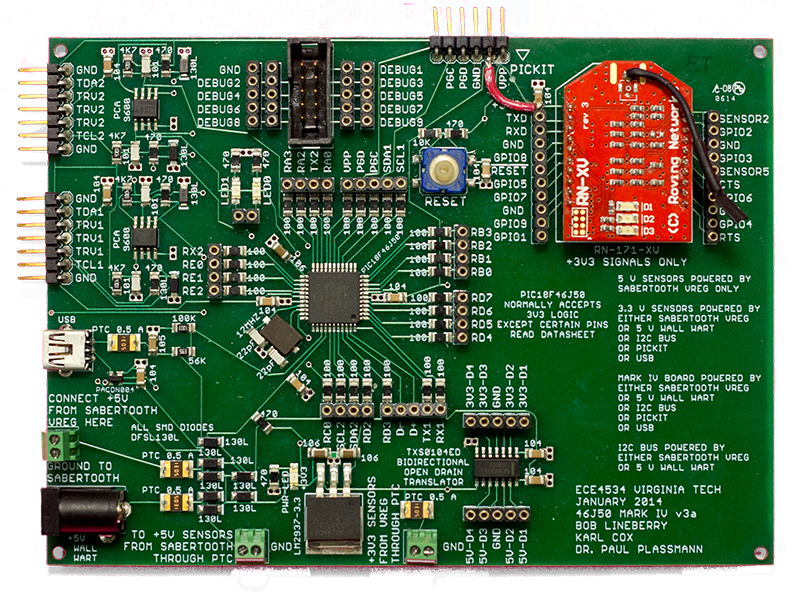
\includegraphics[scale=0.35]{Images/mark4.png}
PIC18F46J50
\end{center}
\begin{center}
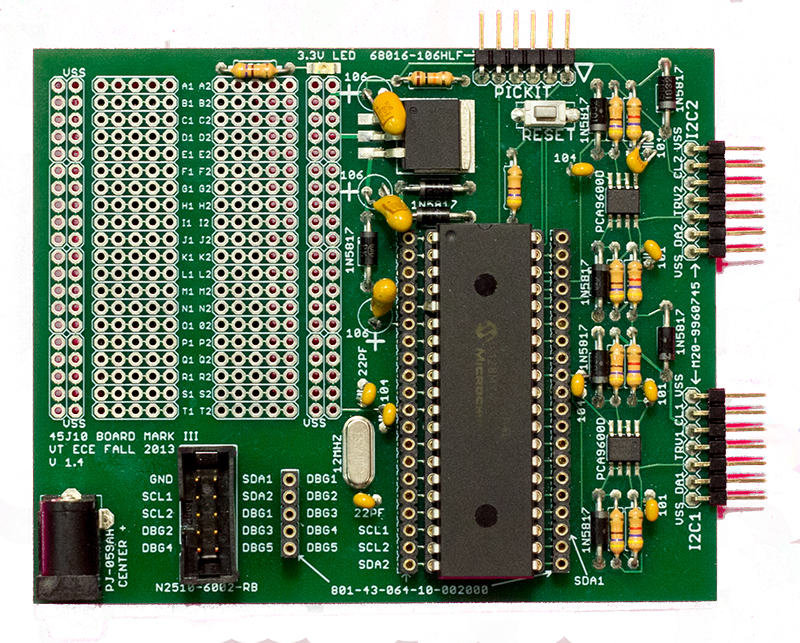
\includegraphics[scale=0.35]{Images/mark3.png}
PIC18F45J10
\end{center}
\begin{center}
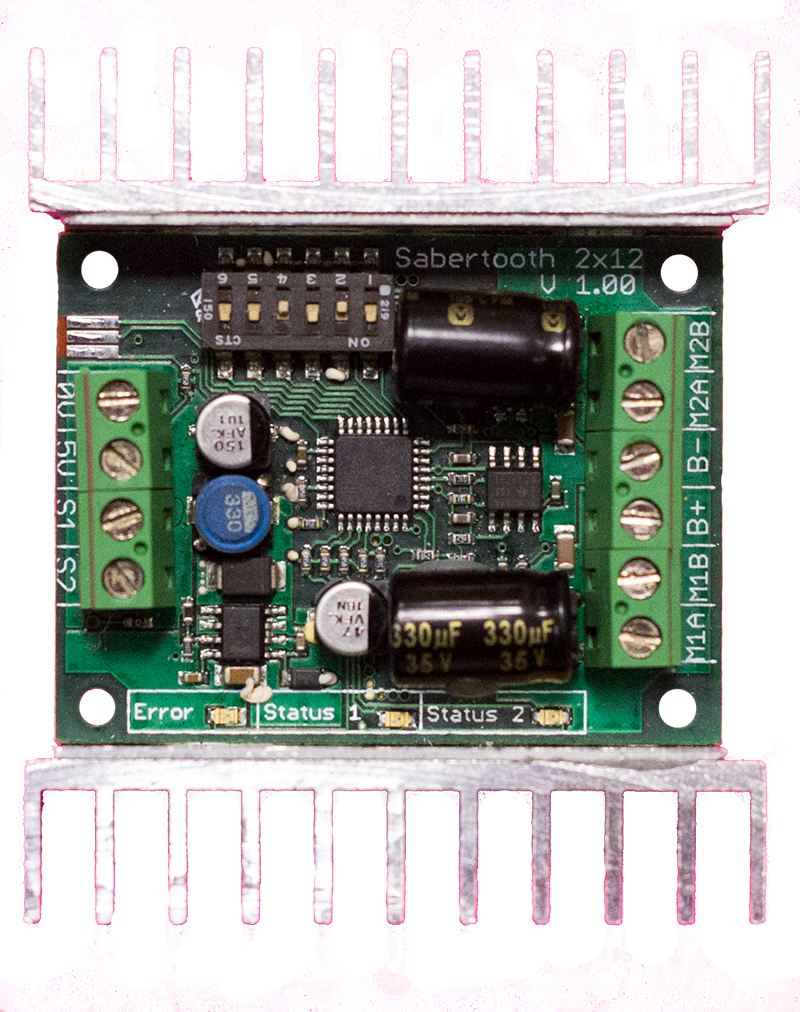
\includegraphics[scale=0.35]{Images/motorcontroller.png}
Sabertooth 2x12 Motor Controller
\end{center}
\begin{center}
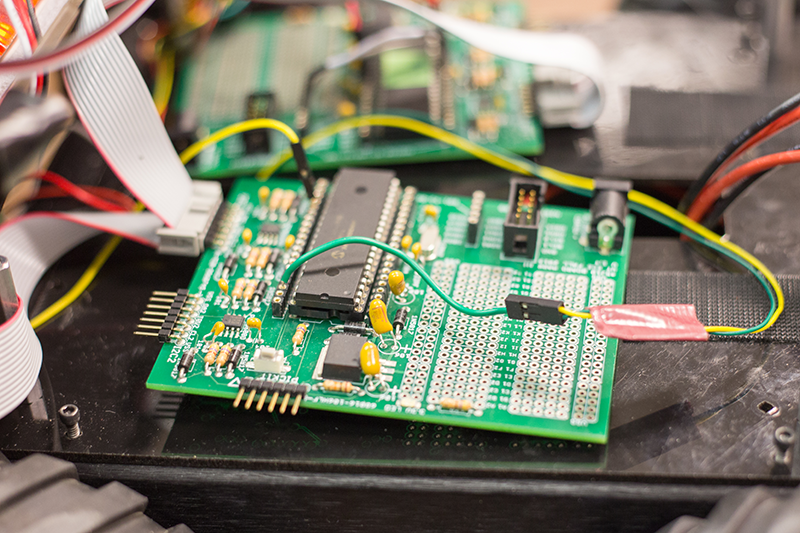
\includegraphics[scale=0.35]{Images/motor.png}
Motor PIC
\end{center}
\begin{center}
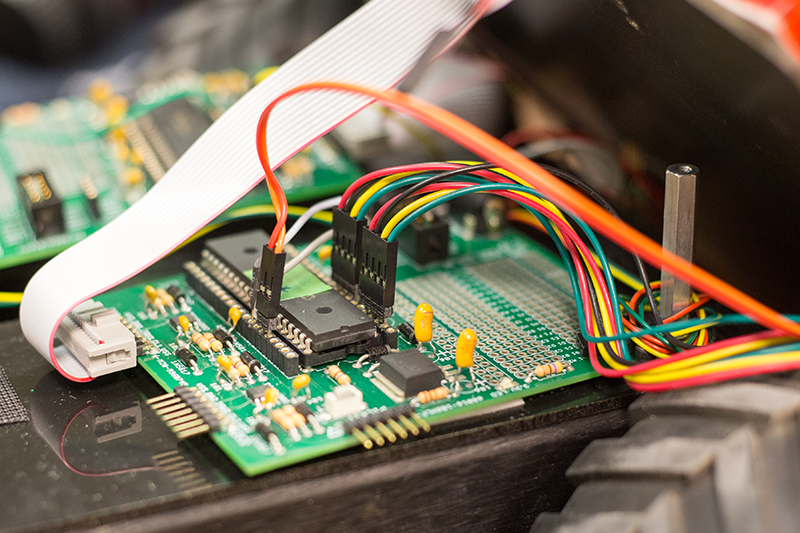
\includegraphics[scale=0.35]{Images/sensor.png}
Sensor PIC
\end{center}
\begin{center}
\includegraphics[scale=0.35]{Images/sensorIP.JPG}
One of the Sensors In Place on the Rover
\end{center}
\begin{center}
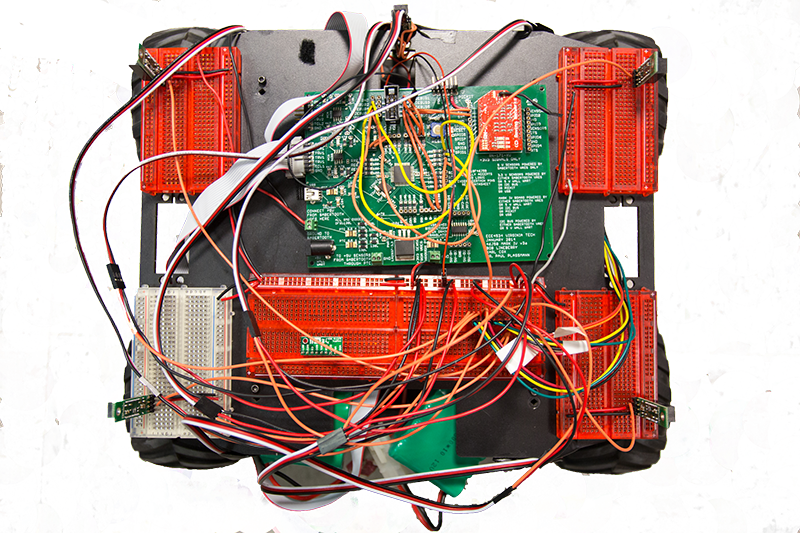
\includegraphics[scale=0.35]{Images/rover.png}
Top view of rover
\end{center}

\subsection{Conclusion}

\end{document}
